\documentclass[1p]{elsarticle_modified}
%\bibliographystyle{elsarticle-num}

%\usepackage[colorlinks]{hyperref}
%\usepackage{abbrmath_seonhwa} %\Abb, \Ascr, \Acal ,\Abf, \Afrak
\usepackage{amsfonts}
\usepackage{amssymb}
\usepackage{amsmath}
\usepackage{amsthm}
\usepackage{scalefnt}
\usepackage{amsbsy}
\usepackage{kotex}
\usepackage{caption}
\usepackage{subfig}
\usepackage{color}
\usepackage{graphicx}
\usepackage{xcolor} %% white, black, red, green, blue, cyan, magenta, yellow
\usepackage{float}
\usepackage{setspace}
\usepackage{hyperref}

\usepackage{tikz}
\usetikzlibrary{arrows}

\usepackage{multirow}
\usepackage{array} % fixed length table
\usepackage{hhline}

%%%%%%%%%%%%%%%%%%%%%
\makeatletter
\renewcommand*\env@matrix[1][\arraystretch]{%
	\edef\arraystretch{#1}%
	\hskip -\arraycolsep
	\let\@ifnextchar\new@ifnextchar
	\array{*\c@MaxMatrixCols c}}
\makeatother %https://tex.stackexchange.com/questions/14071/how-can-i-increase-the-line-spacing-in-a-matrix
%%%%%%%%%%%%%%%

\usepackage[normalem]{ulem}

\newcommand{\msout}[1]{\ifmmode\text{\sout{\ensuremath{#1}}}\else\sout{#1}\fi}
%SOURCE: \msout is \stkout macro in https://tex.stackexchange.com/questions/20609/strikeout-in-math-mode

\newcommand{\cancel}[1]{
	\ifmmode
	{\color{red}\msout{#1}}
	\else
	{\color{red}\sout{#1}}
	\fi
}

\newcommand{\add}[1]{
	{\color{blue}\uwave{#1}}
}

\newcommand{\replace}[2]{
	\ifmmode
	{\color{red}\msout{#1}}{\color{blue}\uwave{#2}}
	\else
	{\color{red}\sout{#1}}{\color{blue}\uwave{#2}}
	\fi
}

\newcommand{\Sol}{\mathcal{S}} %segment
\newcommand{\D}{D} %diagram
\newcommand{\A}{\mathcal{A}} %arc


%%%%%%%%%%%%%%%%%%%%%%%%%%%%%5 test

\def\sl{\operatorname{\textup{SL}}(2,\Cbb)}
\def\psl{\operatorname{\textup{PSL}}(2,\Cbb)}
\def\quan{\mkern 1mu \triangleright \mkern 1mu}

\theoremstyle{definition}
\newtheorem{thm}{Theorem}[section]
\newtheorem{prop}[thm]{Proposition}
\newtheorem{lem}[thm]{Lemma}
\newtheorem{ques}[thm]{Question}
\newtheorem{cor}[thm]{Corollary}
\newtheorem{defn}[thm]{Definition}
\newtheorem{exam}[thm]{Example}
\newtheorem{rmk}[thm]{Remark}
\newtheorem{alg}[thm]{Algorithm}

\newcommand{\I}{\sqrt{-1}}
\begin{document}

%\begin{frontmatter}
%
%\title{Boundary parabolic representations of knots up to 8 crossings}
%
%%% Group authors per affiliation:
%\author{Yunhi Cho} 
%\address{Department of Mathematics, University of Seoul, Seoul, Korea}
%\ead{yhcho@uos.ac.kr}
%
%
%\author{Seonhwa Kim} %\fnref{s_kim}}
%\address{Center for Geometry and Physics, Institute for Basic Science, Pohang, 37673, Korea}
%\ead{ryeona17@ibs.re.kr}
%
%\author{Hyuk Kim}
%\address{Department of Mathematical Sciences, Seoul National University, Seoul 08826, Korea}
%\ead{hyukkim@snu.ac.kr}
%
%\author{Seokbeom Yoon}
%\address{Department of Mathematical Sciences, Seoul National University, Seoul, 08826,  Korea}
%\ead{sbyoon15@snu.ac.kr}
%
%\begin{abstract}
%We find all boundary parabolic representation of knots up to 8 crossings.
%
%\end{abstract}
%\begin{keyword}
%    \MSC[2010] 57M25 
%\end{keyword}
%
%\end{frontmatter}

%\linenumbers
%\tableofcontents
%
\newcommand\colored[1]{\textcolor{white}{\rule[-0.35ex]{0.8em}{1.4ex}}\kern-0.8em\color{red} #1}%
%\newcommand\colored[1]{\textcolor{white}{ #1}\kern-2.17ex	\textcolor{white}{ #1}\kern-1.81ex	\textcolor{white}{ #1}\kern-2.15ex\color{red}#1	}

{\Large $\underline{12a_{0093}~(K12a_{0093})}$}

\setlength{\tabcolsep}{10pt}
\renewcommand{\arraystretch}{1.6}
\vspace{1cm}\begin{tabular}{m{100pt}>{\centering\arraybackslash}m{274pt}}
\multirow{5}{120pt}{
	\centering
	\includegraphics[width=112pt]{../../../GIT/diagram.site/Diagrams/png/894_12a_0093.png}\\
\ \ \ A knot diagram\footnotemark}&
\allowdisplaybreaks
\textbf{Linearized knot diagam} \\
\cline{2-2}
 &
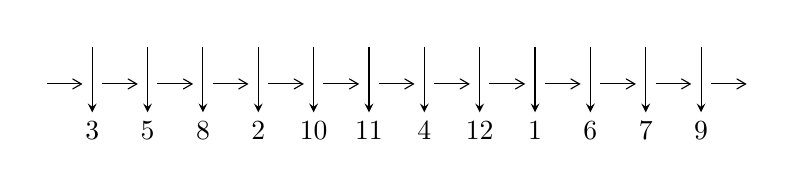
\begin{tikzpicture}[x=20pt, y=17pt]
	% nodes
	\node (C0) at (0, 0) {};
	\node (C1) at (1, 0) {};
	\node (C1U) at (1, +1) {};
	\node (C1D) at (1, -1) {3};

	\node (C2) at (2, 0) {};
	\node (C2U) at (2, +1) {};
	\node (C2D) at (2, -1) {5};

	\node (C3) at (3, 0) {};
	\node (C3U) at (3, +1) {};
	\node (C3D) at (3, -1) {8};

	\node (C4) at (4, 0) {};
	\node (C4U) at (4, +1) {};
	\node (C4D) at (4, -1) {2};

	\node (C5) at (5, 0) {};
	\node (C5U) at (5, +1) {};
	\node (C5D) at (5, -1) {10};

	\node (C6) at (6, 0) {};
	\node (C6U) at (6, +1) {};
	\node (C6D) at (6, -1) {11};

	\node (C7) at (7, 0) {};
	\node (C7U) at (7, +1) {};
	\node (C7D) at (7, -1) {4};

	\node (C8) at (8, 0) {};
	\node (C8U) at (8, +1) {};
	\node (C8D) at (8, -1) {12};

	\node (C9) at (9, 0) {};
	\node (C9U) at (9, +1) {};
	\node (C9D) at (9, -1) {1};

	\node (C10) at (10, 0) {};
	\node (C10U) at (10, +1) {};
	\node (C10D) at (10, -1) {6};

	\node (C11) at (11, 0) {};
	\node (C11U) at (11, +1) {};
	\node (C11D) at (11, -1) {7};

	\node (C12) at (12, 0) {};
	\node (C12U) at (12, +1) {};
	\node (C12D) at (12, -1) {9};
	\node (C13) at (13, 0) {};

	% arrows
	\draw[->,>={angle 60}]
	(C0) edge (C1) (C1) edge (C2) (C2) edge (C3) (C3) edge (C4) (C4) edge (C5) (C5) edge (C6) (C6) edge (C7) (C7) edge (C8) (C8) edge (C9) (C9) edge (C10) (C10) edge (C11) (C11) edge (C12) (C12) edge (C13) ;	\draw[->,>=stealth]
	(C1U) edge (C1D) (C2U) edge (C2D) (C3U) edge (C3D) (C4U) edge (C4D) (C5U) edge (C5D) (C6U) edge (C6D) (C7U) edge (C7D) (C8U) edge (C8D) (C9U) edge (C9D) (C10U) edge (C10D) (C11U) edge (C11D) (C12U) edge (C12D) ;
	\end{tikzpicture} \\
\hhline{~~} \\& 
\textbf{Solving Sequence} \\ \cline{2-2} 
 &
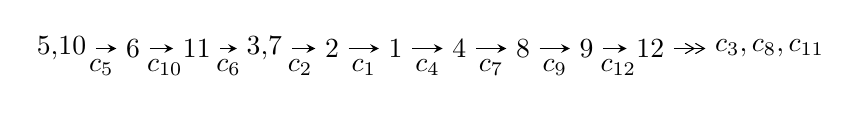
\begin{tikzpicture}[x=23pt, y=7pt]
	% node
	\node (A0) at (-1/8, 0) {5,10};
	\node (A1) at (1, 0) {6};
	\node (A2) at (2, 0) {11};
	\node (A3) at (49/16, 0) {3,7};
	\node (A4) at (33/8, 0) {2};
	\node (A5) at (41/8, 0) {1};
	\node (A6) at (49/8, 0) {4};
	\node (A7) at (57/8, 0) {8};
	\node (A8) at (65/8, 0) {9};
	\node (A9) at (73/8, 0) {12};
	\node (C1) at (1/2, -1) {$c_{5}$};
	\node (C2) at (3/2, -1) {$c_{10}$};
	\node (C3) at (5/2, -1) {$c_{6}$};
	\node (C4) at (29/8, -1) {$c_{2}$};
	\node (C5) at (37/8, -1) {$c_{1}$};
	\node (C6) at (45/8, -1) {$c_{4}$};
	\node (C7) at (53/8, -1) {$c_{7}$};
	\node (C8) at (61/8, -1) {$c_{9}$};
	\node (C9) at (69/8, -1) {$c_{12}$};
	\node (A10) at (11, 0) {$c_{3},c_{8},c_{11}$};

	% edge
	\draw[->,>=stealth]	
	(A0) edge (A1) (A1) edge (A2) (A2) edge (A3) (A3) edge (A4) (A4) edge (A5) (A5) edge (A6) (A6) edge (A7) (A7) edge (A8) (A8) edge (A9) ;
	\draw[->>,>={angle 60}]	
	(A9) edge (A10);
\end{tikzpicture} \\ 

\end{tabular} \\

\footnotetext{
The image of knot diagram is generated by the software ``\textbf{Draw programme}" developed by Andrew Bartholomew(\url{http://www.layer8.co.uk/maths/draw/index.htm\#Running-draw}), where we modified some parts for our purpose(\url{https://github.com/CATsTAILs/LinksPainter}).
}\phantom \\ \newline 
\centering \textbf{Ideals for irreducible components\footnotemark of $X_{\text{par}}$} 
 
\begin{align*}
I^u_{1}&=\langle 
3.70075\times10^{79} u^{71}-3.81232\times10^{79} u^{70}+\cdots+7.87156\times10^{79} b+2.01580\times10^{80},\\
\phantom{I^u_{1}}&\phantom{= \langle  }-2.44050\times10^{79} u^{71}+6.22842\times10^{79} u^{70}+\cdots+1.57431\times10^{80} a-3.01318\times10^{80},\\
\phantom{I^u_{1}}&\phantom{= \langle  }u^{72}-2 u^{71}+\cdots+24 u+8\rangle \\
I^u_{2}&=\langle 
-4 a^2 u+2 a^2+4 a u+7 b+12 a-6 u-4,\;4 a^3-6 a^2 u-8 a^2+2 a u+8 a- u-2,\;u^2-2\rangle \\
I^u_{3}&=\langle 
b+1,\;- u^2+a+u+2,\;u^3- u^2-2 u+1\rangle \\
\\
I^v_{1}&=\langle 
a,\;- v^2+b-3 v+1,\;v^3+2 v^2-3 v+1\rangle \\
\end{align*}
\raggedright * 4 irreducible components of $\dim_{\mathbb{C}}=0$, with total 84 representations.\\
\footnotetext{All coefficients of polynomials are rational numbers. But the coefficients are sometimes approximated in decimal forms when there is not enough margin.}
\newpage
\renewcommand{\arraystretch}{1}
\centering \section*{I. $I^u_{1}= \langle 3.70\times10^{79} u^{71}-3.81\times10^{79} u^{70}+\cdots+7.87\times10^{79} b+2.02\times10^{80},\;-2.44\times10^{79} u^{71}+6.23\times10^{79} u^{70}+\cdots+1.57\times10^{80} a-3.01\times10^{80},\;u^{72}-2 u^{71}+\cdots+24 u+8 \rangle$}
\flushleft \textbf{(i) Arc colorings}\\
\begin{tabular}{m{7pt} m{180pt} m{7pt} m{180pt} }
\flushright $a_{5}=$&$\begin{pmatrix}1\\0\end{pmatrix}$ \\
\flushright $a_{10}=$&$\begin{pmatrix}0\\u\end{pmatrix}$ \\
\flushright $a_{6}=$&$\begin{pmatrix}1\\u^2\end{pmatrix}$ \\
\flushright $a_{11}=$&$\begin{pmatrix}- u\\- u^3+u\end{pmatrix}$ \\
\flushright $a_{3}=$&$\begin{pmatrix}0.155020 u^{71}-0.395628 u^{70}+\cdots-37.7884 u+1.91396\\-0.470142 u^{71}+0.484315 u^{70}+\cdots+4.00972 u-2.56087\end{pmatrix}$ \\
\flushright $a_{7}=$&$\begin{pmatrix}- u^2+1\\- u^4+2 u^2\end{pmatrix}$ \\
\flushright $a_{2}=$&$\begin{pmatrix}-0.315123 u^{71}+0.0886872 u^{70}+\cdots-33.7787 u-0.646903\\-0.470142 u^{71}+0.484315 u^{70}+\cdots+4.00972 u-2.56087\end{pmatrix}$ \\
\flushright $a_{1}=$&$\begin{pmatrix}1.73551 u^{71}-3.17752 u^{70}+\cdots-2.59470 u+17.5888\\-2.40461 u^{71}+2.78349 u^{70}+\cdots+14.3590 u-6.88864\end{pmatrix}$ \\
\flushright $a_{4}=$&$\begin{pmatrix}0.485716 u^{71}-1.14719 u^{70}+\cdots-26.7644 u+3.00194\\-0.981957 u^{71}+1.07115 u^{70}+\cdots+3.98093 u-0.323764\end{pmatrix}$ \\
\flushright $a_{8}=$&$\begin{pmatrix}-0.556973 u^{71}+1.35772 u^{70}+\cdots-20.8031 u-10.0464\\-0.333969 u^{71}-1.38159 u^{70}+\cdots+31.1725 u+18.7963\end{pmatrix}$ \\
\flushright $a_{9}=$&$\begin{pmatrix}0.363304 u^{71}-1.99774 u^{70}+\cdots+35.4662 u+20.3509\\0.618338 u^{71}+1.54449 u^{70}+\cdots-40.5582 u-23.2300\end{pmatrix}$ \\
\flushright $a_{12}=$&$\begin{pmatrix}u^3-2 u\\u^5-3 u^3+u\end{pmatrix}$\\&\end{tabular}
\flushleft \textbf{(ii) Obstruction class $= -1$}\\~\\
\flushleft \textbf{(iii) Cusp Shapes $= 5.63154 u^{71}-8.59389 u^{70}+\cdots-116.925 u-7.71745$}\\~\\
\newpage\renewcommand{\arraystretch}{1}
\flushleft \textbf{(iv) u-Polynomials at the component}\newline \\
\begin{tabular}{m{50pt}|m{274pt}}
Crossings & \hspace{64pt}u-Polynomials at each crossing \\
\hline $$\begin{aligned}c_{1}\end{aligned}$$&$\begin{aligned}
&u^{72}+37 u^{71}+\cdots+107 u+1
\end{aligned}$\\
\hline $$\begin{aligned}c_{2},c_{4}\end{aligned}$$&$\begin{aligned}
&u^{72}-7 u^{71}+\cdots+5 u+1
\end{aligned}$\\
\hline $$\begin{aligned}c_{3},c_{7}\end{aligned}$$&$\begin{aligned}
&u^{72}+2 u^{71}+\cdots+36 u-8
\end{aligned}$\\
\hline $$\begin{aligned}c_{5},c_{6},c_{10}\\c_{11}\end{aligned}$$&$\begin{aligned}
&u^{72}-2 u^{71}+\cdots+24 u+8
\end{aligned}$\\
\hline $$\begin{aligned}c_{8},c_{9},c_{12}\end{aligned}$$&$\begin{aligned}
&u^{72}+5 u^{71}+\cdots+41 u+7
\end{aligned}$\\
\hline
\end{tabular}\\~\\
\newpage\renewcommand{\arraystretch}{1}
\flushleft \textbf{(v) Riley Polynomials at the component}\newline \\
\begin{tabular}{m{50pt}|m{274pt}}
Crossings & \hspace{64pt}Riley Polynomials at each crossing \\
\hline $$\begin{aligned}c_{1}\end{aligned}$$&$\begin{aligned}
&y^{72}+3 y^{71}+\cdots-8427 y+1
\end{aligned}$\\
\hline $$\begin{aligned}c_{2},c_{4}\end{aligned}$$&$\begin{aligned}
&y^{72}-37 y^{71}+\cdots-107 y+1
\end{aligned}$\\
\hline $$\begin{aligned}c_{3},c_{7}\end{aligned}$$&$\begin{aligned}
&y^{72}+30 y^{71}+\cdots-3280 y+64
\end{aligned}$\\
\hline $$\begin{aligned}c_{5},c_{6},c_{10}\\c_{11}\end{aligned}$$&$\begin{aligned}
&y^{72}-88 y^{71}+\cdots-2752 y+64
\end{aligned}$\\
\hline $$\begin{aligned}c_{8},c_{9},c_{12}\end{aligned}$$&$\begin{aligned}
&y^{72}-73 y^{71}+\cdots+1707 y+49
\end{aligned}$\\
\hline
\end{tabular}\\~\\
\newpage\flushleft \textbf{(vi) Complex Volumes and Cusp Shapes}
$$\begin{array}{c|c|c}  
\text{Solutions to }I^u_{1}& \I (\text{vol} + \sqrt{-1}CS) & \text{Cusp shape}\\
 \hline 
\begin{aligned}
u &= -0.875758 + 0.429272 I \\
a &= \phantom{-}0.262678 + 0.101583 I \\
b &= -1.287090 - 0.279824 I\end{aligned}
 & -8.31181 + 2.46798 I & \phantom{-0.000000 } 0 \\ \hline\begin{aligned}
u &= -0.875758 - 0.429272 I \\
a &= \phantom{-}0.262678 - 0.101583 I \\
b &= -1.287090 + 0.279824 I\end{aligned}
 & -8.31181 - 2.46798 I & \phantom{-0.000000 } 0 \\ \hline\begin{aligned}
u &= \phantom{-}0.827261 + 0.504621 I \\
a &= \phantom{-}0.09772 + 2.12500 I \\
b &= -1.121890 - 0.521031 I\end{aligned}
 & -7.76669 - 5.28143 I & \phantom{-0.000000 } 0 \\ \hline\begin{aligned}
u &= \phantom{-}0.827261 - 0.504621 I \\
a &= \phantom{-}0.09772 - 2.12500 I \\
b &= -1.121890 + 0.521031 I\end{aligned}
 & -7.76669 + 5.28143 I & \phantom{-0.000000 } 0 \\ \hline\begin{aligned}
u &= -0.799643 + 0.671253 I \\
a &= \phantom{-}0.06752 + 1.80494 I \\
b &= \phantom{-}1.205120 - 0.572281 I\end{aligned}
 & -6.25612 + 11.79520 I & \phantom{-0.000000 } 0 \\ \hline\begin{aligned}
u &= -0.799643 - 0.671253 I \\
a &= \phantom{-}0.06752 - 1.80494 I \\
b &= \phantom{-}1.205120 + 0.572281 I\end{aligned}
 & -6.25612 - 11.79520 I & \phantom{-0.000000 } 0 \\ \hline\begin{aligned}
u &= -0.744414 + 0.572251 I \\
a &= -0.652228 - 1.062510 I \\
b &= \phantom{-}0.233482 + 0.906675 I\end{aligned}
 & -3.31502 + 6.41563 I & \phantom{-0.000000 } 0 \\ \hline\begin{aligned}
u &= -0.744414 - 0.572251 I \\
a &= -0.652228 + 1.062510 I \\
b &= \phantom{-}0.233482 - 0.906675 I\end{aligned}
 & -3.31502 - 6.41563 I & \phantom{-0.000000 } 0 \\ \hline\begin{aligned}
u &= \phantom{-}0.786461 + 0.477851 I \\
a &= \phantom{-}0.68942 - 1.66417 I \\
b &= \phantom{-}1.084140 + 0.564418 I\end{aligned}
 & \phantom{-}0.01076 - 7.70106 I & \phantom{-0.000000 } 0 \\ \hline\begin{aligned}
u &= \phantom{-}0.786461 - 0.477851 I \\
a &= \phantom{-}0.68942 + 1.66417 I \\
b &= \phantom{-}1.084140 - 0.564418 I\end{aligned}
 & \phantom{-}0.01076 + 7.70106 I & \phantom{-0.000000 } 0\\
 \hline 
 \end{array}$$\newpage$$\begin{array}{c|c|c}  
\text{Solutions to }I^u_{1}& \I (\text{vol} + \sqrt{-1}CS) & \text{Cusp shape}\\
 \hline 
\begin{aligned}
u &= \phantom{-}0.857434 + 0.264670 I \\
a &= \phantom{-}1.02566 - 1.10598 I \\
b &= -0.327725 + 0.634372 I\end{aligned}
 & -5.42751 - 0.70274 I & \phantom{-0.000000 } 0 \\ \hline\begin{aligned}
u &= \phantom{-}0.857434 - 0.264670 I \\
a &= \phantom{-}1.02566 + 1.10598 I \\
b &= -0.327725 - 0.634372 I\end{aligned}
 & -5.42751 + 0.70274 I & \phantom{-0.000000 } 0 \\ \hline\begin{aligned}
u &= -0.879575 + 0.163473 I \\
a &= \phantom{-}1.027390 + 0.651113 I \\
b &= \phantom{-}0.950405 - 0.535597 I\end{aligned}
 & -0.97750 + 2.84413 I & \phantom{-0.000000 } 0 \\ \hline\begin{aligned}
u &= -0.879575 - 0.163473 I \\
a &= \phantom{-}1.027390 - 0.651113 I \\
b &= \phantom{-}0.950405 + 0.535597 I\end{aligned}
 & -0.97750 - 2.84413 I & \phantom{-0.000000 } 0 \\ \hline\begin{aligned}
u &= -0.199773 + 0.851046 I \\
a &= -0.996478 - 0.881875 I \\
b &= \phantom{-}1.147690 + 0.510260 I\end{aligned}
 & -4.44972 - 6.76334 I & -12.00000 + 0. I\phantom{ +0.000000I} \\ \hline\begin{aligned}
u &= -0.199773 - 0.851046 I \\
a &= -0.996478 + 0.881875 I \\
b &= \phantom{-}1.147690 - 0.510260 I\end{aligned}
 & -4.44972 + 6.76334 I & -12.00000 + 0. I\phantom{ +0.000000I} \\ \hline\begin{aligned}
u &= \phantom{-}0.626406 + 0.476151 I \\
a &= -0.717312 + 0.408958 I \\
b &= \phantom{-}0.380216 - 0.718908 I\end{aligned}
 & \phantom{-}2.05866 - 2.81348 I & -9.50002 + 4.98668 I \\ \hline\begin{aligned}
u &= \phantom{-}0.626406 - 0.476151 I \\
a &= -0.717312 - 0.408958 I \\
b &= \phantom{-}0.380216 + 0.718908 I\end{aligned}
 & \phantom{-}2.05866 + 2.81348 I & -9.50002 - 4.98668 I \\ \hline\begin{aligned}
u &= \phantom{-}1.181710 + 0.470204 I \\
a &= -0.1216000 - 0.0229142 I \\
b &= \phantom{-}1.094920 - 0.394215 I\end{aligned}
 & -8.72689 + 2.18989 I & \phantom{-0.000000 } 0 \\ \hline\begin{aligned}
u &= \phantom{-}1.181710 - 0.470204 I \\
a &= -0.1216000 + 0.0229142 I \\
b &= \phantom{-}1.094920 + 0.394215 I\end{aligned}
 & -8.72689 - 2.18989 I & \phantom{-0.000000 } 0\\
 \hline 
 \end{array}$$\newpage$$\begin{array}{c|c|c}  
\text{Solutions to }I^u_{1}& \I (\text{vol} + \sqrt{-1}CS) & \text{Cusp shape}\\
 \hline 
\begin{aligned}
u &= -0.611935 + 0.376277 I \\
a &= -0.283350 + 0.621830 I \\
b &= \phantom{-}0.649429 + 0.513270 I\end{aligned}
 & -0.07524 - 1.41658 I & -12.97255 + 1.10740 I \\ \hline\begin{aligned}
u &= -0.611935 - 0.376277 I \\
a &= -0.283350 - 0.621830 I \\
b &= \phantom{-}0.649429 - 0.513270 I\end{aligned}
 & -0.07524 + 1.41658 I & -12.97255 - 1.10740 I \\ \hline\begin{aligned}
u &= -0.214744 + 0.682258 I \\
a &= \phantom{-}0.40025 + 1.69752 I \\
b &= \phantom{-}0.197456 - 0.697303 I\end{aligned}
 & -1.72777 - 2.16585 I & -11.52549 + 1.08940 I \\ \hline\begin{aligned}
u &= -0.214744 - 0.682258 I \\
a &= \phantom{-}0.40025 - 1.69752 I \\
b &= \phantom{-}0.197456 + 0.697303 I\end{aligned}
 & -1.72777 + 2.16585 I & -11.52549 - 1.08940 I \\ \hline\begin{aligned}
u &= \phantom{-}0.054234 + 0.691316 I \\
a &= \phantom{-}1.57683 - 1.56133 I \\
b &= -1.142460 + 0.370676 I\end{aligned}
 & -5.43584 + 1.26277 I & -16.3916 - 0.1881 I \\ \hline\begin{aligned}
u &= \phantom{-}0.054234 - 0.691316 I \\
a &= \phantom{-}1.57683 + 1.56133 I \\
b &= -1.142460 - 0.370676 I\end{aligned}
 & -5.43584 - 1.26277 I & -16.3916 + 0.1881 I \\ \hline\begin{aligned}
u &= -0.617110 + 0.307371 I \\
a &= -0.59785 - 2.50870 I \\
b &= -0.986315 + 0.384932 I\end{aligned}
 & -2.03116 + 2.58391 I & -16.3746 - 6.6287 I \\ \hline\begin{aligned}
u &= -0.617110 - 0.307371 I \\
a &= -0.59785 + 2.50870 I \\
b &= -0.986315 - 0.384932 I\end{aligned}
 & -2.03116 - 2.58391 I & -16.3746 + 6.6287 I \\ \hline\begin{aligned}
u &= \phantom{-}0.276521 + 0.561410 I \\
a &= -0.19398 - 1.44729 I \\
b &= \phantom{-}0.600878 + 0.650005 I\end{aligned}
 & \phantom{-}3.08581 - 0.76384 I & -6.34873 + 2.59077 I \\ \hline\begin{aligned}
u &= \phantom{-}0.276521 - 0.561410 I \\
a &= -0.19398 + 1.44729 I \\
b &= \phantom{-}0.600878 - 0.650005 I\end{aligned}
 & \phantom{-}3.08581 + 0.76384 I & -6.34873 - 2.59077 I\\
 \hline 
 \end{array}$$\newpage$$\begin{array}{c|c|c}  
\text{Solutions to }I^u_{1}& \I (\text{vol} + \sqrt{-1}CS) & \text{Cusp shape}\\
 \hline 
\begin{aligned}
u &= -1.396880 + 0.035985 I \\
a &= \phantom{-}0.186911 + 0.763642 I \\
b &= \phantom{-}0.831473 - 0.725123 I\end{aligned}
 & -1.87165 + 2.75314 I & \phantom{-0.000000 } 0 \\ \hline\begin{aligned}
u &= -1.396880 - 0.035985 I \\
a &= \phantom{-}0.186911 - 0.763642 I \\
b &= \phantom{-}0.831473 + 0.725123 I\end{aligned}
 & -1.87165 - 2.75314 I & \phantom{-0.000000 } 0 \\ \hline\begin{aligned}
u &= -1.40156\phantom{ +0.000000I} \\
a &= \phantom{-}11.4734\phantom{ +0.000000I} \\
b &= -0.988970\phantom{ +0.000000I}\end{aligned}
 & -8.19953\phantom{ +0.000000I} & \phantom{-0.000000 } 0 \\ \hline\begin{aligned}
u &= \phantom{-}0.092090 + 0.573260 I \\
a &= -0.770057 + 1.161670 I \\
b &= \phantom{-}0.953023 - 0.598994 I\end{aligned}
 & \phantom{-}2.06822 + 4.08017 I & -7.94616 - 5.26935 I \\ \hline\begin{aligned}
u &= \phantom{-}0.092090 - 0.573260 I \\
a &= -0.770057 - 1.161670 I \\
b &= \phantom{-}0.953023 + 0.598994 I\end{aligned}
 & \phantom{-}2.06822 - 4.08017 I & -7.94616 + 5.26935 I \\ \hline\begin{aligned}
u &= \phantom{-}0.550545 + 0.163361 I \\
a &= -1.57695 + 0.17909 I \\
b &= -1.110070 + 0.163246 I\end{aligned}
 & -2.56966 - 0.57818 I & -16.8714 + 8.9218 I \\ \hline\begin{aligned}
u &= \phantom{-}0.550545 - 0.163361 I \\
a &= -1.57695 - 0.17909 I \\
b &= -1.110070 - 0.163246 I\end{aligned}
 & -2.56966 + 0.57818 I & -16.8714 - 8.9218 I \\ \hline\begin{aligned}
u &= \phantom{-}1.42095 + 0.21273 I \\
a &= \phantom{-}0.542378 - 0.597190 I \\
b &= \phantom{-}0.590617 + 0.161261 I\end{aligned}
 & -6.67741 - 0.58823 I & \phantom{-0.000000 } 0 \\ \hline\begin{aligned}
u &= \phantom{-}1.42095 - 0.21273 I \\
a &= \phantom{-}0.542378 + 0.597190 I \\
b &= \phantom{-}0.590617 - 0.161261 I\end{aligned}
 & -6.67741 + 0.58823 I & \phantom{-0.000000 } 0 \\ \hline\begin{aligned}
u &= \phantom{-}1.47025\phantom{ +0.000000I} \\
a &= \phantom{-}0.911193\phantom{ +0.000000I} \\
b &= -0.327218\phantom{ +0.000000I}\end{aligned}
 & -6.78796\phantom{ +0.000000I} & \phantom{-0.000000 } 0\\
 \hline 
 \end{array}$$\newpage$$\begin{array}{c|c|c}  
\text{Solutions to }I^u_{1}& \I (\text{vol} + \sqrt{-1}CS) & \text{Cusp shape}\\
 \hline 
\begin{aligned}
u &= -0.481111 + 0.095743 I \\
a &= -0.79648 + 1.70877 I \\
b &= \phantom{-}0.865855 - 0.831513 I\end{aligned}
 & \phantom{-}0.90495 + 3.07172 I & -20.6395 - 5.9253 I \\ \hline\begin{aligned}
u &= -0.481111 - 0.095743 I \\
a &= -0.79648 - 1.70877 I \\
b &= \phantom{-}0.865855 + 0.831513 I\end{aligned}
 & \phantom{-}0.90495 - 3.07172 I & -20.6395 + 5.9253 I \\ \hline\begin{aligned}
u &= \phantom{-}1.53498 + 0.03198 I \\
a &= \phantom{-}0.438335 + 0.164331 I \\
b &= -0.058233 - 0.496424 I\end{aligned}
 & -6.93072 - 0.11771 I & \phantom{-0.000000 } 0 \\ \hline\begin{aligned}
u &= \phantom{-}1.53498 - 0.03198 I \\
a &= \phantom{-}0.438335 - 0.164331 I \\
b &= -0.058233 + 0.496424 I\end{aligned}
 & -6.93072 + 0.11771 I & \phantom{-0.000000 } 0 \\ \hline\begin{aligned}
u &= \phantom{-}1.58385 + 0.02369 I \\
a &= -0.055937 - 0.975650 I \\
b &= \phantom{-}0.910185 + 0.970380 I\end{aligned}
 & -6.39453 - 3.47846 I & \phantom{-0.000000 } 0 \\ \hline\begin{aligned}
u &= \phantom{-}1.58385 - 0.02369 I \\
a &= -0.055937 + 0.975650 I \\
b &= \phantom{-}0.910185 - 0.970380 I\end{aligned}
 & -6.39453 + 3.47846 I & \phantom{-0.000000 } 0 \\ \hline\begin{aligned}
u &= -1.58359 + 0.12100 I \\
a &= -0.233603 - 0.250046 I \\
b &= \phantom{-}0.219437 + 0.848024 I\end{aligned}
 & -5.41979 + 4.93889 I & \phantom{-0.000000 } 0 \\ \hline\begin{aligned}
u &= -1.58359 - 0.12100 I \\
a &= -0.233603 + 0.250046 I \\
b &= \phantom{-}0.219437 - 0.848024 I\end{aligned}
 & -5.41979 - 4.93889 I & \phantom{-0.000000 } 0 \\ \hline\begin{aligned}
u &= -1.58812 + 0.03042 I \\
a &= -1.228490 + 0.430142 I \\
b &= -1.230760 - 0.307392 I\end{aligned}
 & -10.01110 + 1.19025 I & \phantom{-0.000000 } 0 \\ \hline\begin{aligned}
u &= -1.58812 - 0.03042 I \\
a &= -1.228490 - 0.430142 I \\
b &= -1.230760 + 0.307392 I\end{aligned}
 & -10.01110 - 1.19025 I & \phantom{-0.000000 } 0\\
 \hline 
 \end{array}$$\newpage$$\begin{array}{c|c|c}  
\text{Solutions to }I^u_{1}& \I (\text{vol} + \sqrt{-1}CS) & \text{Cusp shape}\\
 \hline 
\begin{aligned}
u &= \phantom{-}1.59443 + 0.07004 I \\
a &= -0.95915 + 1.33782 I \\
b &= -1.126480 - 0.469683 I\end{aligned}
 & -9.64311 - 3.88422 I & \phantom{-0.000000 } 0 \\ \hline\begin{aligned}
u &= \phantom{-}1.59443 - 0.07004 I \\
a &= -0.95915 - 1.33782 I \\
b &= -1.126480 + 0.469683 I\end{aligned}
 & -9.64311 + 3.88422 I & \phantom{-0.000000 } 0 \\ \hline\begin{aligned}
u &= -0.395087\phantom{ +0.000000I} \\
a &= \phantom{-}0.927031\phantom{ +0.000000I} \\
b &= -0.104752\phantom{ +0.000000I}\end{aligned}
 & -0.588530\phantom{ +0.000000I} & -16.7510\phantom{ +0.000000I} \\ \hline\begin{aligned}
u &= -0.221019 + 0.289419 I \\
a &= \phantom{-}2.12036 + 0.93378 I \\
b &= -0.778490 - 0.216174 I\end{aligned}
 & -0.944244 - 0.257791 I & -11.16562 - 1.59535 I \\ \hline\begin{aligned}
u &= -0.221019 - 0.289419 I \\
a &= \phantom{-}2.12036 - 0.93378 I \\
b &= -0.778490 + 0.216174 I\end{aligned}
 & -0.944244 + 0.257791 I & -11.16562 + 1.59535 I \\ \hline\begin{aligned}
u &= \phantom{-}1.62768 + 0.17150 I \\
a &= -0.431502 + 0.570990 I \\
b &= \phantom{-}0.243814 - 1.044500 I\end{aligned}
 & -11.3658 - 9.2318 I & \phantom{-0.000000 } 0 \\ \hline\begin{aligned}
u &= \phantom{-}1.62768 - 0.17150 I \\
a &= -0.431502 - 0.570990 I \\
b &= \phantom{-}0.243814 + 1.044500 I\end{aligned}
 & -11.3658 + 9.2318 I & \phantom{-0.000000 } 0 \\ \hline\begin{aligned}
u &= -1.64174 + 0.14153 I \\
a &= \phantom{-}0.96072 + 1.05427 I \\
b &= \phantom{-}1.188910 - 0.551097 I\end{aligned}
 & -8.31688 + 10.07720 I & \phantom{-0.000000 } 0 \\ \hline\begin{aligned}
u &= -1.64174 - 0.14153 I \\
a &= \phantom{-}0.96072 - 1.05427 I \\
b &= \phantom{-}1.188910 + 0.551097 I\end{aligned}
 & -8.31688 - 10.07720 I & \phantom{-0.000000 } 0 \\ \hline\begin{aligned}
u &= -1.64839 + 0.08124 I \\
a &= \phantom{-}0.477835 + 0.762351 I \\
b &= -0.442405 - 0.890711 I\end{aligned}
 & -14.0714 + 2.0898 I & \phantom{-0.000000 } 0\\
 \hline 
 \end{array}$$\newpage$$\begin{array}{c|c|c}  
\text{Solutions to }I^u_{1}& \I (\text{vol} + \sqrt{-1}CS) & \text{Cusp shape}\\
 \hline 
\begin{aligned}
u &= -1.64839 - 0.08124 I \\
a &= \phantom{-}0.477835 - 0.762351 I \\
b &= -0.442405 + 0.890711 I\end{aligned}
 & -14.0714 - 2.0898 I & \phantom{-0.000000 } 0 \\ \hline\begin{aligned}
u &= -1.65163 + 0.14342 I \\
a &= -0.41603 - 1.43600 I \\
b &= -1.153970 + 0.638956 I\end{aligned}
 & -16.2646 + 7.7641 I & \phantom{-0.000000 } 0 \\ \hline\begin{aligned}
u &= -1.65163 - 0.14342 I \\
a &= -0.41603 + 1.43600 I \\
b &= -1.153970 - 0.638956 I\end{aligned}
 & -16.2646 - 7.7641 I & \phantom{-0.000000 } 0 \\ \hline\begin{aligned}
u &= \phantom{-}1.64915 + 0.20871 I \\
a &= \phantom{-}0.65126 - 1.32967 I \\
b &= \phantom{-}1.260260 + 0.616858 I\end{aligned}
 & -14.5211 - 15.1783 I & \phantom{-0.000000 } 0 \\ \hline\begin{aligned}
u &= \phantom{-}1.64915 - 0.20871 I \\
a &= \phantom{-}0.65126 + 1.32967 I \\
b &= \phantom{-}1.260260 - 0.616858 I\end{aligned}
 & -14.5211 + 15.1783 I & \phantom{-0.000000 } 0 \\ \hline\begin{aligned}
u &= \phantom{-}1.65979 + 0.11678 I \\
a &= -0.486333 - 0.039718 I \\
b &= -1.41864 + 0.27823 I\end{aligned}
 & -17.0477 - 4.5612 I & \phantom{-0.000000 } 0 \\ \hline\begin{aligned}
u &= \phantom{-}1.65979 - 0.11678 I \\
a &= -0.486333 + 0.039718 I \\
b &= -1.41864 - 0.27823 I\end{aligned}
 & -17.0477 + 4.5612 I & \phantom{-0.000000 } 0 \\ \hline\begin{aligned}
u &= \phantom{-}1.66435 + 0.06433 I \\
a &= \phantom{-}1.010600 - 0.515375 I \\
b &= \phantom{-}1.126480 + 0.439828 I\end{aligned}
 & -9.85240 - 3.84777 I & \phantom{-0.000000 } 0 \\ \hline\begin{aligned}
u &= \phantom{-}1.66435 - 0.06433 I \\
a &= \phantom{-}1.010600 + 0.515375 I \\
b &= \phantom{-}1.126480 - 0.439828 I\end{aligned}
 & -9.85240 + 3.84777 I & \phantom{-0.000000 } 0 \\ \hline\begin{aligned}
u &= \phantom{-}0.229806\phantom{ +0.000000I} \\
a &= -13.4178\phantom{ +0.000000I} \\
b &= -0.871083\phantom{ +0.000000I}\end{aligned}
 & -2.90601\phantom{ +0.000000I} & -61.9330\phantom{ +0.000000I}\\
 \hline 
 \end{array}$$\newpage$$\begin{array}{c|c|c}  
\text{Solutions to }I^u_{1}& \I (\text{vol} + \sqrt{-1}CS) & \text{Cusp shape}\\
 \hline 
\begin{aligned}
u &= -1.78412 + 0.04723 I \\
a &= \phantom{-}0.534525 - 0.028315 I \\
b &= \phantom{-}1.096760 + 0.161668 I\end{aligned}
 & -19.6154 - 0.2070 I & \phantom{-0.000000 } 0 \\ \hline\begin{aligned}
u &= -1.78412 - 0.04723 I \\
a &= \phantom{-}0.534525 + 0.028315 I \\
b &= \phantom{-}1.096760 - 0.161668 I\end{aligned}
 & -19.6154 + 0.2070 I & \phantom{-0.000000 } 0\\
 \hline 
 \end{array}$$\newpage\newpage\renewcommand{\arraystretch}{1}
\centering \section*{II. $I^u_{2}= \langle -4 a^2 u+2 a^2+4 a u+7 b+12 a-6 u-4,\;4 a^3-6 a^2 u-8 a^2+2 a u+8 a- u-2,\;u^2-2 \rangle$}
\flushleft \textbf{(i) Arc colorings}\\
\begin{tabular}{m{7pt} m{180pt} m{7pt} m{180pt} }
\flushright $a_{5}=$&$\begin{pmatrix}1\\0\end{pmatrix}$ \\
\flushright $a_{10}=$&$\begin{pmatrix}0\\u\end{pmatrix}$ \\
\flushright $a_{6}=$&$\begin{pmatrix}1\\2\end{pmatrix}$ \\
\flushright $a_{11}=$&$\begin{pmatrix}- u\\- u\end{pmatrix}$ \\
\flushright $a_{3}=$&$\begin{pmatrix}a\\\frac{4}{7} a^2 u-\frac{4}{7} a u+\cdots-\frac{12}{7} a+\frac{4}{7}\end{pmatrix}$ \\
\flushright $a_{7}=$&$\begin{pmatrix}-1\\0\end{pmatrix}$ \\
\flushright $a_{2}=$&$\begin{pmatrix}\frac{4}{7} a^2 u-\frac{4}{7} a u+\cdots-\frac{5}{7} a+\frac{4}{7}\\\frac{4}{7} a^2 u-\frac{4}{7} a u+\cdots-\frac{12}{7} a+\frac{4}{7}\end{pmatrix}$ \\
\flushright $a_{1}=$&$\begin{pmatrix}\frac{1}{2} u\\\frac{2}{7} a^2 u+\frac{5}{7} a u+\cdots+\frac{8}{7} a+\frac{2}{7}\end{pmatrix}$ \\
\flushright $a_{4}=$&$\begin{pmatrix}-\frac{3}{7} a^2 u+\frac{10}{7} a u+\cdots+\frac{16}{7} a-\frac{3}{7}\\-\frac{2}{7} a^2 u+\frac{9}{7} a u+\cdots+\frac{20}{7} a-\frac{9}{7}\end{pmatrix}$ \\
\flushright $a_{8}=$&$\begin{pmatrix}\frac{1}{2} u\\\frac{2}{7} a^2 u+\frac{5}{7} a u+\cdots+\frac{8}{7} a+\frac{2}{7}\end{pmatrix}$ \\
\flushright $a_{9}=$&$\begin{pmatrix}\frac{1}{2} u\\\frac{2}{7} a^2 u+\frac{5}{7} a u+\cdots+\frac{8}{7} a+\frac{2}{7}\end{pmatrix}$ \\
\flushright $a_{12}=$&$\begin{pmatrix}0\\- u\end{pmatrix}$\\&\end{tabular}
\flushleft \textbf{(ii) Obstruction class $= 1$}\\~\\
\flushleft \textbf{(iii) Cusp Shapes $= \frac{16}{7} a^2 u-\frac{8}{7} a^2-\frac{16}{7} a u-\frac{48}{7} a+\frac{24}{7} u-\frac{124}{7}$}\\~\\
\newpage\renewcommand{\arraystretch}{1}
\flushleft \textbf{(iv) u-Polynomials at the component}\newline \\
\begin{tabular}{m{50pt}|m{274pt}}
Crossings & \hspace{64pt}u-Polynomials at each crossing \\
\hline $$\begin{aligned}c_{1},c_{7}\end{aligned}$$&$\begin{aligned}
&(u^3- u^2+2 u-1)^2
\end{aligned}$\\
\hline $$\begin{aligned}c_{2}\end{aligned}$$&$\begin{aligned}
&(u^3+u^2-1)^2
\end{aligned}$\\
\hline $$\begin{aligned}c_{3}\end{aligned}$$&$\begin{aligned}
&(u^3+u^2+2 u+1)^2
\end{aligned}$\\
\hline $$\begin{aligned}c_{4}\end{aligned}$$&$\begin{aligned}
&(u^3- u^2+1)^2
\end{aligned}$\\
\hline $$\begin{aligned}c_{5},c_{6},c_{10}\\c_{11}\end{aligned}$$&$\begin{aligned}
&(u^2-2)^3
\end{aligned}$\\
\hline $$\begin{aligned}c_{8},c_{9}\end{aligned}$$&$\begin{aligned}
&(u+1)^6
\end{aligned}$\\
\hline $$\begin{aligned}c_{12}\end{aligned}$$&$\begin{aligned}
&(u-1)^6
\end{aligned}$\\
\hline
\end{tabular}\\~\\
\newpage\renewcommand{\arraystretch}{1}
\flushleft \textbf{(v) Riley Polynomials at the component}\newline \\
\begin{tabular}{m{50pt}|m{274pt}}
Crossings & \hspace{64pt}Riley Polynomials at each crossing \\
\hline $$\begin{aligned}c_{1},c_{3},c_{7}\end{aligned}$$&$\begin{aligned}
&(y^3+3 y^2+2 y-1)^2
\end{aligned}$\\
\hline $$\begin{aligned}c_{2},c_{4}\end{aligned}$$&$\begin{aligned}
&(y^3- y^2+2 y-1)^2
\end{aligned}$\\
\hline $$\begin{aligned}c_{5},c_{6},c_{10}\\c_{11}\end{aligned}$$&$\begin{aligned}
&(y-2)^6
\end{aligned}$\\
\hline $$\begin{aligned}c_{8},c_{9},c_{12}\end{aligned}$$&$\begin{aligned}
&(y-1)^6
\end{aligned}$\\
\hline
\end{tabular}\\~\\
\newpage\flushleft \textbf{(vi) Complex Volumes and Cusp Shapes}
$$\begin{array}{c|c|c}  
\text{Solutions to }I^u_{2}& \I (\text{vol} + \sqrt{-1}CS) & \text{Cusp shape}\\
 \hline 
\begin{aligned}
u &= \phantom{-}1.41421\phantom{ +0.000000I} \\
a &= \phantom{-}0.361309 + 0.347270 I \\
b &= \phantom{-}0.877439 - 0.744862 I\end{aligned}
 & -3.55561 + 2.82812 I & -16.4902 - 2.9794 I \\ \hline\begin{aligned}
u &= \phantom{-}1.41421\phantom{ +0.000000I} \\
a &= \phantom{-}0.361309 - 0.347270 I \\
b &= \phantom{-}0.877439 + 0.744862 I\end{aligned}
 & -3.55561 - 2.82812 I & -16.4902 + 2.9794 I \\ \hline\begin{aligned}
u &= \phantom{-}1.41421\phantom{ +0.000000I} \\
a &= \phantom{-}3.39870\phantom{ +0.000000I} \\
b &= -0.754878\phantom{ +0.000000I}\end{aligned}
 & -7.69319\phantom{ +0.000000I} & -23.0200\phantom{ +0.000000I} \\ \hline\begin{aligned}
u &= -1.41421\phantom{ +0.000000I} \\
a &= -0.116187 + 1.142450 I \\
b &= \phantom{-}0.877439 - 0.744862 I\end{aligned}
 & -3.55561 + 2.82812 I & -16.4902 - 2.9794 I \\ \hline\begin{aligned}
u &= -1.41421\phantom{ +0.000000I} \\
a &= -0.116187 - 1.142450 I \\
b &= \phantom{-}0.877439 + 0.744862 I\end{aligned}
 & -3.55561 - 2.82812 I & -16.4902 + 2.9794 I \\ \hline\begin{aligned}
u &= -1.41421\phantom{ +0.000000I} \\
a &= \phantom{-}0.111054\phantom{ +0.000000I} \\
b &= -0.754878\phantom{ +0.000000I}\end{aligned}
 & -7.69319\phantom{ +0.000000I} & -23.0200\phantom{ +0.000000I}\\
 \hline 
 \end{array}$$\newpage\newpage\renewcommand{\arraystretch}{1}
\centering \section*{III. $I^u_{3}= \langle b+1,\;- u^2+a+u+2,\;u^3- u^2-2 u+1 \rangle$}
\flushleft \textbf{(i) Arc colorings}\\
\begin{tabular}{m{7pt} m{180pt} m{7pt} m{180pt} }
\flushright $a_{5}=$&$\begin{pmatrix}1\\0\end{pmatrix}$ \\
\flushright $a_{10}=$&$\begin{pmatrix}0\\u\end{pmatrix}$ \\
\flushright $a_{6}=$&$\begin{pmatrix}1\\u^2\end{pmatrix}$ \\
\flushright $a_{11}=$&$\begin{pmatrix}- u\\- u^2- u+1\end{pmatrix}$ \\
\flushright $a_{3}=$&$\begin{pmatrix}u^2- u-2\\-1\end{pmatrix}$ \\
\flushright $a_{7}=$&$\begin{pmatrix}- u^2+1\\- u^2- u+1\end{pmatrix}$ \\
\flushright $a_{2}=$&$\begin{pmatrix}u^2- u-3\\-1\end{pmatrix}$ \\
\flushright $a_{1}=$&$\begin{pmatrix}-1\\0\end{pmatrix}$ \\
\flushright $a_{4}=$&$\begin{pmatrix}u^2- u-2\\-1\end{pmatrix}$ \\
\flushright $a_{8}=$&$\begin{pmatrix}- u^2+1\\- u^2- u+1\end{pmatrix}$ \\
\flushright $a_{9}=$&$\begin{pmatrix}u\\u\end{pmatrix}$ \\
\flushright $a_{12}=$&$\begin{pmatrix}u^2-1\\u^2\end{pmatrix}$\\&\end{tabular}
\flushleft \textbf{(ii) Obstruction class $= 1$}\\~\\
\flushleft \textbf{(iii) Cusp Shapes $= u^2+4 u-16$}\\~\\
\newpage\renewcommand{\arraystretch}{1}
\flushleft \textbf{(iv) u-Polynomials at the component}\newline \\
\begin{tabular}{m{50pt}|m{274pt}}
Crossings & \hspace{64pt}u-Polynomials at each crossing \\
\hline $$\begin{aligned}c_{1},c_{2}\end{aligned}$$&$\begin{aligned}
&(u-1)^3
\end{aligned}$\\
\hline $$\begin{aligned}c_{3},c_{7}\end{aligned}$$&$\begin{aligned}
&u^3
\end{aligned}$\\
\hline $$\begin{aligned}c_{4}\end{aligned}$$&$\begin{aligned}
&(u+1)^3
\end{aligned}$\\
\hline $$\begin{aligned}c_{5},c_{6},c_{8}\\c_{9}\end{aligned}$$&$\begin{aligned}
&u^3- u^2-2 u+1
\end{aligned}$\\
\hline $$\begin{aligned}c_{10},c_{11},c_{12}\end{aligned}$$&$\begin{aligned}
&u^3+u^2-2 u-1
\end{aligned}$\\
\hline
\end{tabular}\\~\\
\newpage\renewcommand{\arraystretch}{1}
\flushleft \textbf{(v) Riley Polynomials at the component}\newline \\
\begin{tabular}{m{50pt}|m{274pt}}
Crossings & \hspace{64pt}Riley Polynomials at each crossing \\
\hline $$\begin{aligned}c_{1},c_{2},c_{4}\end{aligned}$$&$\begin{aligned}
&(y-1)^3
\end{aligned}$\\
\hline $$\begin{aligned}c_{3},c_{7}\end{aligned}$$&$\begin{aligned}
&y^3
\end{aligned}$\\
\hline $$\begin{aligned}c_{5},c_{6},c_{8}\\c_{9},c_{10},c_{11}\\c_{12}\end{aligned}$$&$\begin{aligned}
&y^3-5 y^2+6 y-1
\end{aligned}$\\
\hline
\end{tabular}\\~\\
\newpage\flushleft \textbf{(vi) Complex Volumes and Cusp Shapes}
$$\begin{array}{c|c|c}  
\text{Solutions to }I^u_{3}& \I (\text{vol} + \sqrt{-1}CS) & \text{Cusp shape}\\
 \hline 
\begin{aligned}
u &= -1.24698\phantom{ +0.000000I} \\
a &= \phantom{-}0.801938\phantom{ +0.000000I} \\
b &= -1.00000\phantom{ +0.000000I}\end{aligned}
 & -7.98968\phantom{ +0.000000I} & -19.4330\phantom{ +0.000000I} \\ \hline\begin{aligned}
u &= \phantom{-}0.445042\phantom{ +0.000000I} \\
a &= -2.24698\phantom{ +0.000000I} \\
b &= -1.00000\phantom{ +0.000000I}\end{aligned}
 & -2.34991\phantom{ +0.000000I} & -14.0220\phantom{ +0.000000I} \\ \hline\begin{aligned}
u &= \phantom{-}1.80194\phantom{ +0.000000I} \\
a &= -0.554958\phantom{ +0.000000I} \\
b &= -1.00000\phantom{ +0.000000I}\end{aligned}
 & -19.2692\phantom{ +0.000000I} & -5.54530\phantom{ +0.000000I}\\
 \hline 
 \end{array}$$\newpage\newpage\renewcommand{\arraystretch}{1}
\centering \section*{IV. $I^v_{1}= \langle a,\;- v^2+b-3 v+1,\;v^3+2 v^2-3 v+1 \rangle$}
\flushleft \textbf{(i) Arc colorings}\\
\begin{tabular}{m{7pt} m{180pt} m{7pt} m{180pt} }
\flushright $a_{5}=$&$\begin{pmatrix}1\\0\end{pmatrix}$ \\
\flushright $a_{10}=$&$\begin{pmatrix}v\\0\end{pmatrix}$ \\
\flushright $a_{6}=$&$\begin{pmatrix}1\\0\end{pmatrix}$ \\
\flushright $a_{11}=$&$\begin{pmatrix}v\\0\end{pmatrix}$ \\
\flushright $a_{3}=$&$\begin{pmatrix}0\\v^2+3 v-1\end{pmatrix}$ \\
\flushright $a_{7}=$&$\begin{pmatrix}1\\0\end{pmatrix}$ \\
\flushright $a_{2}=$&$\begin{pmatrix}v^2+3 v-1\\v^2+3 v-1\end{pmatrix}$ \\
\flushright $a_{1}=$&$\begin{pmatrix}v^2+3 v-1\\- v^2-2 v+3\end{pmatrix}$ \\
\flushright $a_{4}=$&$\begin{pmatrix}-2 v^2-5 v+4\\-2 v^2-5 v+3\end{pmatrix}$ \\
\flushright $a_{8}=$&$\begin{pmatrix}- v^2-3 v+1\\v^2+2 v-3\end{pmatrix}$ \\
\flushright $a_{9}=$&$\begin{pmatrix}- v^2-2 v+1\\v^2+2 v-3\end{pmatrix}$ \\
\flushright $a_{12}=$&$\begin{pmatrix}v\\0\end{pmatrix}$\\&\end{tabular}
\flushleft \textbf{(ii) Obstruction class $= 1$}\\~\\
\flushleft \textbf{(iii) Cusp Shapes $= -2 v-6$}\\~\\
\newpage\renewcommand{\arraystretch}{1}
\flushleft \textbf{(iv) u-Polynomials at the component}\newline \\
\begin{tabular}{m{50pt}|m{274pt}}
Crossings & \hspace{64pt}u-Polynomials at each crossing \\
\hline $$\begin{aligned}c_{1},c_{3}\end{aligned}$$&$\begin{aligned}
&u^3- u^2+2 u-1
\end{aligned}$\\
\hline $$\begin{aligned}c_{2}\end{aligned}$$&$\begin{aligned}
&u^3+u^2-1
\end{aligned}$\\
\hline $$\begin{aligned}c_{4}\end{aligned}$$&$\begin{aligned}
&u^3- u^2+1
\end{aligned}$\\
\hline $$\begin{aligned}c_{5},c_{6},c_{10}\\c_{11}\end{aligned}$$&$\begin{aligned}
&u^3
\end{aligned}$\\
\hline $$\begin{aligned}c_{7}\end{aligned}$$&$\begin{aligned}
&u^3+u^2+2 u+1
\end{aligned}$\\
\hline $$\begin{aligned}c_{8},c_{9}\end{aligned}$$&$\begin{aligned}
&(u-1)^3
\end{aligned}$\\
\hline $$\begin{aligned}c_{12}\end{aligned}$$&$\begin{aligned}
&(u+1)^3
\end{aligned}$\\
\hline
\end{tabular}\\~\\
\newpage\renewcommand{\arraystretch}{1}
\flushleft \textbf{(v) Riley Polynomials at the component}\newline \\
\begin{tabular}{m{50pt}|m{274pt}}
Crossings & \hspace{64pt}Riley Polynomials at each crossing \\
\hline $$\begin{aligned}c_{1},c_{3},c_{7}\end{aligned}$$&$\begin{aligned}
&y^3+3 y^2+2 y-1
\end{aligned}$\\
\hline $$\begin{aligned}c_{2},c_{4}\end{aligned}$$&$\begin{aligned}
&y^3- y^2+2 y-1
\end{aligned}$\\
\hline $$\begin{aligned}c_{5},c_{6},c_{10}\\c_{11}\end{aligned}$$&$\begin{aligned}
&y^3
\end{aligned}$\\
\hline $$\begin{aligned}c_{8},c_{9},c_{12}\end{aligned}$$&$\begin{aligned}
&(y-1)^3
\end{aligned}$\\
\hline
\end{tabular}\\~\\
\newpage\flushleft \textbf{(vi) Complex Volumes and Cusp Shapes}
$$\begin{array}{c|c|c}  
\text{Solutions to }I^v_{1}& \I (\text{vol} + \sqrt{-1}CS) & \text{Cusp shape}\\
 \hline 
\begin{aligned}
v &= \phantom{-}0.539798 + 0.182582 I \\
a &= \phantom{-0.000000 } 0 \\
b &= \phantom{-}0.877439 + 0.744862 I\end{aligned}
 & \phantom{-}1.37919 - 2.82812 I & -7.07960 - 0.36516 I \\ \hline\begin{aligned}
v &= \phantom{-}0.539798 - 0.182582 I \\
a &= \phantom{-0.000000 } 0 \\
b &= \phantom{-}0.877439 - 0.744862 I\end{aligned}
 & \phantom{-}1.37919 + 2.82812 I & -7.07960 + 0.36516 I \\ \hline\begin{aligned}
v &= -3.07960\phantom{ +0.000000I} \\
a &= \phantom{-0.000000 } 0 \\
b &= -0.754878\phantom{ +0.000000I}\end{aligned}
 & -2.75839\phantom{ +0.000000I} & \phantom{-}0.159190\phantom{ +0.000000I}\\
 \hline 
 \end{array}$$\newpage
\newpage\renewcommand{\arraystretch}{1}
\centering \section*{ V. u-Polynomials}
\begin{tabular}{m{50pt}|m{274pt}}
Crossings & \hspace{64pt}u-Polynomials at each crossing \\
\hline $$\begin{aligned}c_{1}\end{aligned}$$&$\begin{aligned}
&((u-1)^3)(u^3- u^2+2 u-1)^3(u^{72}+37 u^{71}+\cdots+107 u+1)
\end{aligned}$\\
\hline $$\begin{aligned}c_{2}\end{aligned}$$&$\begin{aligned}
&((u-1)^3)(u^3+u^2-1)^3(u^{72}-7 u^{71}+\cdots+5 u+1)
\end{aligned}$\\
\hline $$\begin{aligned}c_{3}\end{aligned}$$&$\begin{aligned}
&u^3(u^3- u^2+2 u-1)(u^3+u^2+2 u+1)^{2}(u^{72}+2 u^{71}+\cdots+36 u-8)
\end{aligned}$\\
\hline $$\begin{aligned}c_{4}\end{aligned}$$&$\begin{aligned}
&((u+1)^3)(u^3- u^2+1)^3(u^{72}-7 u^{71}+\cdots+5 u+1)
\end{aligned}$\\
\hline $$\begin{aligned}c_{5},c_{6}\end{aligned}$$&$\begin{aligned}
&u^3(u^2-2)^3(u^3- u^2-2 u+1)(u^{72}-2 u^{71}+\cdots+24 u+8)
\end{aligned}$\\
\hline $$\begin{aligned}c_{7}\end{aligned}$$&$\begin{aligned}
&u^3(u^3- u^2+2 u-1)^{2}(u^3+u^2+2 u+1)(u^{72}+2 u^{71}+\cdots+36 u-8)
\end{aligned}$\\
\hline $$\begin{aligned}c_{8},c_{9}\end{aligned}$$&$\begin{aligned}
&((u-1)^3)(u+1)^6(u^3- u^2-2 u+1)(u^{72}+5 u^{71}+\cdots+41 u+7)
\end{aligned}$\\
\hline $$\begin{aligned}c_{10},c_{11}\end{aligned}$$&$\begin{aligned}
&u^3(u^2-2)^3(u^3+u^2-2 u-1)(u^{72}-2 u^{71}+\cdots+24 u+8)
\end{aligned}$\\
\hline $$\begin{aligned}c_{12}\end{aligned}$$&$\begin{aligned}
&((u-1)^6)(u+1)^3(u^3+u^2-2 u-1)(u^{72}+5 u^{71}+\cdots+41 u+7)
\end{aligned}$\\
\hline
\end{tabular}\newpage\renewcommand{\arraystretch}{1}
\centering \section*{ VI. Riley Polynomials}
\begin{tabular}{m{50pt}|m{274pt}}
Crossings & \hspace{64pt}Riley Polynomials at each crossing \\
\hline $$\begin{aligned}c_{1}\end{aligned}$$&$\begin{aligned}
&((y-1)^3)(y^3+3 y^2+2 y-1)^3(y^{72}+3 y^{71}+\cdots-8427 y+1)
\end{aligned}$\\
\hline $$\begin{aligned}c_{2},c_{4}\end{aligned}$$&$\begin{aligned}
&((y-1)^3)(y^3- y^2+2 y-1)^3(y^{72}-37 y^{71}+\cdots-107 y+1)
\end{aligned}$\\
\hline $$\begin{aligned}c_{3},c_{7}\end{aligned}$$&$\begin{aligned}
&y^3(y^3+3 y^2+2 y-1)^3(y^{72}+30 y^{71}+\cdots-3280 y+64)
\end{aligned}$\\
\hline $$\begin{aligned}c_{5},c_{6},c_{10}\\c_{11}\end{aligned}$$&$\begin{aligned}
&y^3(y-2)^6(y^{3}-5 y^{2}+6 y-1)(y^{72}-88 y^{71}+\cdots-2752 y+64)
\end{aligned}$\\
\hline $$\begin{aligned}c_{8},c_{9},c_{12}\end{aligned}$$&$\begin{aligned}
&((y-1)^9)(y^3-5 y^2+6 y-1)(y^{72}-73 y^{71}+\cdots+1707 y+49)
\end{aligned}$\\
\hline
\end{tabular}
\vskip 2pc
\end{document}